\documentclass[11pt]{beamer}
\usetheme{default}

\usepackage{fontspec}
\usepackage[spanish, es-nodecimaldot]{babel}
\usepackage{amsmath}
\usepackage{amsfonts}
\usepackage{amssymb}
\usepackage{graphicx}
\usepackage{url}

\usepackage{amsmath}
\usepackage{xparse}
\usepackage{amsthm}
\usepackage{tikz}

% Seno
\def\sen{\mathop{\mbox{\normalfont sen}}\nolimits}

% Seno hiperbólico
\def\senh{\mathop{\mbox{\normalfont senh}}\nolimits}

% Arcoseno
\def\arcsen{\mathop{\mbox{\normalfont arcsen}}\nolimits}

% Gradiente
\def\grad{\mathop{\mbox{\normalfont grad}}\nolimits}

% Argumento principal
\def\Arg{\mathop{\mbox{\normalfont Arg}}\nolimits}

% Logaritmo complejo
\def\Log{\mathop{\mbox{\normalfont Log}}\nolimits}

% Rotacional
\def\rot{\mathop{\mbox{\normalfont rot}}\nolimits}

% Divergencia
\def\diver{\mathop{\mbox{\normalfont div}}\nolimits}

% Longitud
\def\longi{\mathop{\mbox{\normalfont long}}\nolimits}

% Índice de una curva
\def\ind{\mathop{\mbox{\normalfont Ind}}\nolimits}

% Rango de una matriz
\def\rang{\mathop{\mbox{\normalfont rang}}\nolimits}

% Norma
\newcommand{\norm}[1]{\lVert #1 \rVert}

% Derivada parcial
\newcommand{\derpar}[1]{\dfrac{\partial}{\partial #1}}

% Derivada parcial con función
\newcommand{\derparcial}[2]{\dfrac{\partial #1}{\partial #2}}

% Derivada parcial de orden n con funcion
\newcommand{\derparcialn}[3]{\dfrac{\partial^{#3} #1}{\partial #2^{#3}}}

% Integral doble en [a,b] x [c,d]
\newcommand{\intdob}[4]{\displaystyle \int_{#1}^{#2} \int_{#3}^{#4}}

% Integral triple en [a,b] x [c,d] x [e,f]
\newcommand{\inttri}[6]{\displaystyle \int_{#1}^{#2} \int_{#3}^{#4} \int_{#5}^{#6}}

% Números complejos
\def\C{\ensuremath{\mathbb{C}}}

% Números reales
\def\R{\ensuremath{\mathbb{R}}}

% Números racionales
\def\Q{\ensuremath{\mathbb{Q}}}

% Números enteros
\def\Z{\ensuremath{\mathbb{Z}}}

% Números naturales
\def\N{\ensuremath{\mathbb{N}}}

% Teorema
\newtheorem{teo}{Teorema}

% Corolario
\newtheorem{cor}{Corolario}

% Proposición
\newtheorem{prop}{Proposición}

% Lema
\newtheorem{lema}{Lema}

% Definición
\newtheorem{defi}{Definición}

% Observaciones
\newtheorem*{obs}{Observaciones}

\newtheorem*{ob}{Observación}

\newtheorem*{nota}{Nota}

\newtheorem*{problema}{Problema}

\newtheorem*{pregunta}{Pregunta}

\newtheorem{ejemplo}{Ejemplo}

\NewDocumentCommand{\overarrow}{O{=} O{\uparrow} m}{%
  \overset{\makebox[0pt]{\begin{tabular}{@{}c@{}}#3\\[0pt]\ensuremath{#2}\end{tabular}}}{#1}
}
\NewDocumentCommand{\underarrow}{O{=} O{\downarrow} m}{%
  \underset{\makebox[0pt]{\begin{tabular}{@{}c@{}}\ensuremath{#2}\\[0pt]#3\end{tabular}}}{\ensuremath{#1}}
}

\newcommand{\contradiction}{%
\begin{tikzpicture}[rotate=45,x=0.5ex,y=0.5ex]
\draw[color=red, line width=.1ex] (0,2) -- (3,2) (0,1) -- (3,1) (1,3) -- (1,0) (2,3) -- (2,0);
\end{tikzpicture}
}

\usepackage{pgf}
\usepackage{tikz}
\usetikzlibrary{arrows,automata}

\newcommand{\ejemplografo}{
\begin{tikzpicture}[>=stealth',shorten >=1pt,auto,node distance=3cm,semithick]
  \tikzstyle{every state}=[draw=black,text=black]

  \node[state]         (A)                    {$A$};
  \node[state]         (B) [right of=A]       {$B$};
  \node[state]         (C) [below of=A]       {$C$};
  \node[state]         (D) [right of=C]       {$D$};
  
  \path (A) edge  [bend left]   node {}  (B)
            edge  [bend right]  node {}  (C)
        (B) edge                node {}  (C)
        (C) edge  [bend right]  node {}  (D);
\end{tikzpicture}}

\newcommand{\ejemplografocompleto}{
\begin{tikzpicture}[>=stealth',shorten >=1pt,auto,node distance=3cm,semithick]
  \tikzstyle{every state}=[draw=black,text=black]

  \node[state]         (A)                    {$A$};
  \node[state]         (B) [right of=A]       {$B$};
  \node[state]         (C) [below of=A]       {$C$};
  \node[state]         (D) [right of=C]       {$D$};
  
  \path (A) edge  [bend left]   node {}  (B)
            edge  [bend right]  node {}  (C)
		(B) edge  [bend left]   node {}  (D)
        (B) edge                node {}  (C)
        (D) edge                node {}  (A)
        (C) edge  [bend right]  node {}  (D);
\end{tikzpicture}}

\newcommand{\ejemplografodirigido}{
\begin{tikzpicture}[->,>=stealth',shorten >=1pt,auto,node distance=3cm,semithick]
  \tikzstyle{every state}=[draw=black,text=black]

  \node[state]         (A)                    {$A$};
  \node[state]         (B) [right of=A]       {$B$};
  \node[state]         (C) [below of=A]       {$C$};
  \node[state]         (D) [right of=C]       {$D$};
  
  \path (A) edge  [bend left]   node {}  (B)
            edge  [bend right]  node {}  (C)
        (B) edge                node {}  (C)
        (C) edge  [bend right]  node  {}  (D)
        (C) edge  [loop below]  node  {}  (C);
\end{tikzpicture}}

\newcommand{\ejemplosubgrafo}{
\begin{tikzpicture}[>=stealth',shorten >=1pt,auto,node distance=2cm,semithick]
  \tikzstyle{every state}=[draw=black,text=black]

% Grafo G
  \node[state]         (E)                          {$E$};
  \node[state]         (B) [above right of=E]       {$B$};
  \node[state]         (A) [above left of= E]       {$A$};
  \node[state]         (C) [below left of= E]       {$C$};
  \node[state]         (D) [below right of=E]       {$D$};

  \path (A) edge                node {}  (B)
        (A) edge                node {}  (E)
        (A) edge                node {}  (C)
        (B) edge                node {}  (D)
        (B) edge                node {}  (E)        
        (C) edge                node {}  (E)
        (C) edge                node {}  (D)
        (D) edge                node {}  (E);
        
        
% Subgrafo G'
  \node[state]         (F) [right of= B]       {$A$};
  \node[state]         (G) [right of= F]       {$B$};
  \node[state]         (H) [right of= D]       {$C$};
  \node[state]         (I) [right of= H]       {$D$};
  
  \path (F) edge                node {}  (G)
        (F) edge                node {}  (H)
        (G) edge                node {}  (I)
        (H) edge                node {}  (I);
        
% Subgrafo G'

  \node[state]         (J) [right of= G]             {$A$};
  \node[state]         (K) [right of= I]             {$C$};
  \node[state]         (N) [above right of= K]       {$E$};
  \node[state]         (M) [below right of= N]       {$D$};
  \node[state]         (L) [above right of= N]       {$B$};
  
  \path (J) edge                node {}  (K)
        (J) edge                node {}  (L)
        (L) edge                node {}  (N)
        (L) edge                node {}  (M)
        (K) edge                node {}  (M);
        
% Etiquetas con el nombre de los grafos
  \node[align=center, below right of=C] {$G$};
  \node[align=center, below right of=H] {$G'$};
  \node[align=center, below right of=K] {$G''$};
\end{tikzpicture}}

\newcommand{\ejemplounionintersecciongrafo}{
\begin{tikzpicture}[>=stealth',shorten >=1pt,auto,node distance=2cm,semithick]
  \tikzstyle{every state}=[draw=black,text=black]

% Grafo G
  \node[state]         (A)                          {$A$};
  \node[state]         (B) [below right of=A]       {$B$};
  \node[state]         (C) [below      of= B]       {$C$};
  \node[state]         (D) [right of=B]             {$D$};
  \node[state]         (E) [right of=C]             {$E$};

  \path (A) edge                node {}  (B)
        (B) edge                node {}  (C)
        (B) edge                node {}  (D)      
        (C) edge                node {}  (E)
        (D) edge                node {}  (E);
        
% Grafo G'
  \node[state]         (H) [right of= E]       {$C$};
  \node[state]         (I) [right of= D]       {$D$};
  \node[state]         (G) [right of= H]       {$E$};
  \node[state]         (F) [above right of= G] {$F$};
  
  \path (H) edge                node {}  (I)
        (I) edge                node {}  (F)
        (G) edge                node {}  (F)
        (H) edge                node {}  (G);
        
% Etiquetas con el nombre de los grafos
  \node[align=center, below right of=C] (Z) {$G$};
  \node[align=center, below right of=H] (Y) {$G'$};

% Grafo G \cup G'
  \node[state]         (J) [below left of=Z]        {$A$};
  \node[state]         (K) [below right of=J]       {$B$};
  \node[state]         (L) [below of= K]            {$C$};
  \node[state]         (M) [right of=K]             {$D$};
  \node[state]         (N) [right of=L]             {$E$};
  \node[state]         (R) [above right of=N]       {$F$};

  \path (J) edge                node {}  (K)
        (K) edge                node {}  (L)
        (K) edge                node {}  (M)      
        (L) edge                node {}  (N)
        (L) edge                node {}  (M)
        (N) edge                node {}  (R)
        (R) edge                node {}  (M)
        (M) edge                node {}  (N);
        
  \node[align=center, below right of=L] {$G \cup G'$};
  
% Grafo G \cup G'
  \node[state]         (O) [right of=R]        {$C$};
  \node[state]         (P) [right of=O]              {$E$};


  \path (O) edge                node {}  (P);
        
        
  \node[align=center, below right of=O] {$G \cap G'$};

\end{tikzpicture}}


\newcommand{\ejemplomarkov}{
\begin{tikzpicture}[->,>=stealth',shorten >=1pt,auto,node distance=5cm,semithick]
  \tikzstyle{every state}=[draw=black,text=black]

  \node[state]         (A)                    {$A$};
  \node[state]         (B) [below left of=A]  {$B$};
  \node[state]         (C) [below right of=A] {$C$};
  
  \path (A) edge  [loop above] node {$0.65$} (A)
            edge  [bend left]  node {$0.3$}  (B)
            edge  [bend left]  node {$0.05$} (C)
        (B) edge  [loop below] node {$0.75$} (B)
            edge  [bend left]  node {$0.1$}  (A)
            edge               node {$0.15$} (C)
        (C) edge  [loop below] node {$0.8$}  (C)
            edge  [bend left]  node {$0.01$} (A)
            edge  [bend left]  node {$0.19$} (B);
\end{tikzpicture}}

\newcommand{\ejemplomarkovcompleto}{
\begin{tikzpicture}[->,>=stealth',shorten >=1pt,auto,node distance=5cm,semithick]
  \tikzstyle{every state}=[draw=black,text=black]

  \node[state]         (S)                    {$S$};
  \node[state]         (H)      [right of=A]  {$H$};
  
  \path (S) edge  [loop above] node {$0.5$}  (S)
            edge  [bend left]  node {$0.5$}  (H)
        (H) edge  [loop below] node {$0.75$} (H)
            edge  [bend left]  node {$0.25$} (S);

\end{tikzpicture}}



\author{José Ignacio Escribano}
\title{Diseño e implementación de una aplicación SPA para el estudio de la competitividad de la liga BBVA}
%\subtitle{}
%\logo{}
\institute{URJC}
\date{}
%\subject{}
\setbeamercovered{transparent}
\setbeamertemplate{navigation symbols}{}

\setsansfont[Ligatures=TeX]{texgyreadventor}
\setmainfont[Ligatures=TeX]{texgyrepagella}

\begin{document}
	
	\begin{frame}
		\maketitle
	\end{frame}

	\begin{frame}[allowframebreaks]{Índice}
		\tableofcontents
	\end{frame}
	
	
	\section{Introducción}
	
	\begin{frame}{Introducción}
		Vivimos rodeados de rankings
		
		\begin{itemize}
			\item Rankings socioeconómicos
			\begin{itemize}
				\item Producto Interior Bruto
				\item Prima de riesgo
				\item Igualdad de ingreso
			\end{itemize}
			\item Rankings deportivos
			\begin{itemize}
				\item En fútbol, el ranking FIFA
				\item En tenis, el ranking ATP/WTA
				\item En baloncesto, el draft de la NBA
			\end{itemize}
			\item Etc.
		\end{itemize}
	\end{frame}
	
	\begin{frame}{Introducción}
		\begin{figure}
			\centering
			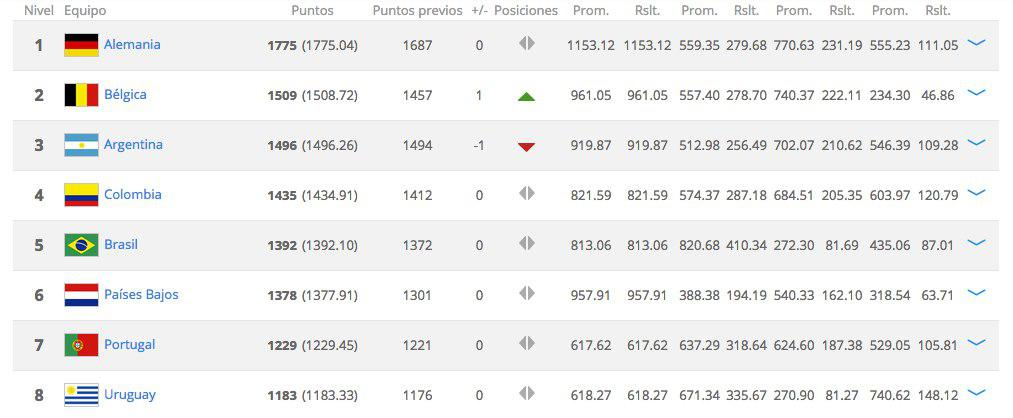
\includegraphics[width=0.9\linewidth]{imagenes/ranking_fifa}
			\caption{Ranking FIFA \url{http://es.fifa.com/fifa-world-ranking/ranking-table/men/}}
			\label{fig:ranking_fifa}
		\end{figure}
	\end{frame}
	
	\begin{frame}{Introducción}
		\begin{figure}
			\centering
			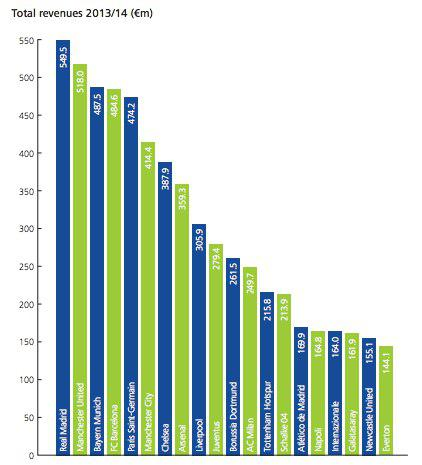
\includegraphics[width=0.5\linewidth]{imagenes/ranking_deloitte}
			\caption{Football Money League \url{http://www2.deloitte.com/content/dam/Deloitte/uk/Documents/sports-business-group/deloitte-football-money-league-2015.PDF}}
			\label{fig:ranking_deloitte}
		\end{figure}
	\end{frame}
	
	\begin{frame}{Introducción}
		\begin{figure}
			\centering
			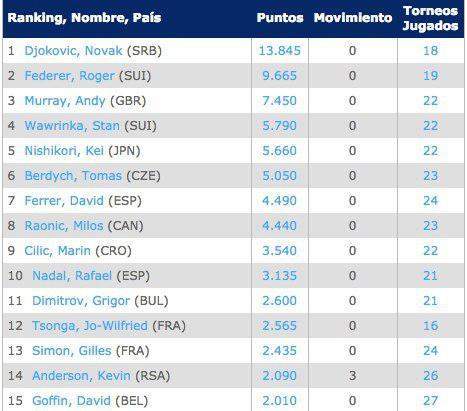
\includegraphics[width=0.7\linewidth]{imagenes/ranking_atp}
			\caption{Ranking ATP \url{http://es.atpworldtour.com/Rankings/Singles.aspx}}
			\label{fig:ranking_atp}
		\end{figure}
	\end{frame}
	
	\subsection{¿Qué un rating? ¿Y un ranking?}
	
	\begin{frame}{¿Qué un rating?}
		\begin{defi}
			Dado un conjunto $\mathcal{N} = \{1,\dots, n\}$ de nodos, decimos que es un rating si a cada $i \in \mathcal{N}$ se le asigna un valor real, es decir, una función $\mathrm{r} : \mathcal{N} \to \R$.
		\end{defi}
	\end{frame}
	
	\begin{frame}{¿Qué un ranking?}
		\begin{defi} \label{def:ranking}
			Dado un conjunto $\mathcal{N} = \{1,\dots,n\}$ que llamamos nodos, definimos el ranking $c$ como cualquier biyección $c : \mathcal{N} \to \mathcal{N}$.
		\end{defi}
		
		Un rating cuando se ordena (ascendente o descendentemente), crea un ranking.
	\end{frame}
	
	\begin{frame}{¿Qué es un ranking?}
		Otra forma de ver los rankings y los ratings es en forma de vector. Si tenemos un ranking $c$, cada una de las posiciones del vector $c$, se corresponde con alguno de los nodos, y la posición en la aparezca en el vector es la posición que tiene en el ranking $c$. De igual forma para un rating.
		
		\begin{ejemplo}
			$$ c = \left(
			\begin{array}{c}
			\text{Equipo } 1 \\
			\text{Equipo } 4 \\
			\text{Equipo } 2 \\
			\vdots \\
			\text{Equipo } n
			\end{array}
			\right) $$
				
			En el ranking $c$ el Equipo $1$ ocupa la primera posición, el Equipo $4$ ocupa la segunda posición, el Equipo 2 la tercera posición y así sucesivamente.
			
		\end{ejemplo}
	\end{frame}
	
	\section{Métodos para obtener ratings (y rankings)}
	
	\begin{frame}{Métodos para obtener ratings (y rankings)}
		Existen muchos métodos para obtener ratings. Sólo veremos tres métodos:
		
		\begin{itemize}
			\item Método de Massey: basado en mínimos cuadrados
			\item Método de Colley: basado en la regla de Laplace
			\item Método de Markov: basado en cadenas de Markov
		\end{itemize}
	\end{frame}
	
	\subsection{Método de Massey}
	
	\begin{frame}{Método de Massey}
		Basado en la siguiente ecuación idealizada:
		
		\begin{equation}
		r_i - r_j = y_k
		\end{equation} 
		
		donde $y_k$ es el margen de victoria para el partido $k$, y $r_i$ y $r_j$ son los ratings de los equipos $i$ y $j$, respectivamente. En otras palabras, la diferencia de los ratings $r_i$ y $r_j$ de dos equipos predice idealmente el margen de victoria en un enfrentamiento entre estos dos equipos.
	
	\end{frame}
	
	\begin{frame}{Método de Massey}
	
		Se puede expresar de la forma 
		
		\[ \mathbf{M r} = \mathbf{p} \]
		
		donde $\mathbf{M}$ es la matriz formada en la diagonal con 
		
	\end{frame}
	
	\subsection{Método de Colley}
	
	\begin{frame}{Método de Colley}
		Método de Colley
	\end{frame}
	
	\subsection{Método de Markov}
	
	\begin{frame}{Método de Markov}
		Método de Markov
	\end{frame}
	
	\section{Agregación de rankings}
	
	\begin{frame}{Agregación de rankings}
		En la práctica, se tienen distintos rankings sobre un misma estadística con resultados totalmente distintos.\\
		
		Es recomendable agregar todos esos rankings iniciales para crear un nuevo ranking que contenga la información de todos esos rankings iniciales.\\
		
		Hay que destacar que si partimos de rankings con buena calidad, obtendremos un buen ranking agregado. De la misma forma, si tenemos unos malos rankings iniciales, obtendremos un ranking agregado de mala calidad.
	\end{frame}
	
	\begin{frame}{Agregación de rankings}
		\begin{figure}
			\centering
			\agregacionrankings
			\caption{Agregación de rankings}
			\label{fig:agregación_rankings}
		\end{figure}
	\end{frame}
	
	\subsection{Métodos de agregación de rankings}
	
	\subsubsection{Método de Borda}
	
	\begin{frame}{Método de Borda}
		
		\begin{itemize}
			\item Para cada ranking, cada equipo recibe una puntuación igual al número de equipos que le superan.
			
			\item La puntuación de cada ranking es sumada para cada equipo para crear un nuevo ranking, que se llama recuento de Borda.
			
			\item Los equipos son ordenados en orden ascendente según este método para obtener el ranking.
		\end{itemize}
		
	\end{frame}
	
	\begin{frame}{Método de Borda}
		
		Ejemplo del método
		
	\end{frame}
	
	\subsubsection{Método del ranking promedio}
	
	\begin{frame}{Método del ranking promedio}
		\begin{itemize}
			\item Los números enteros que representan el orden en el ranking en los distintos rankings, se hace la media aritmética con éstos para crear el nuevo ranking agregado.
			
			\item Sólo es válido para rankings completos (rankings con el mismo número de elementos).
		\end{itemize}
	\end{frame}
	
	\begin{frame}{Método del ranking promedio}
		Ejemplo	Método del ranking promedio
	\end{frame}
	
	\subsubsection{Método de datos de partidos simulados}
	
	\begin{frame}{Método de datos de partidos simulados}
		\begin{figure}
			\centering
			\resizebox{.6\linewidth}{!}{\partidossimulados}
			
			\caption{Método de datos de partidos simulados}
			\label{fig:partidos_simulados}
		\end{figure}
	\end{frame}
	
	\subsubsection{Método óptimo de agregación de rankings}
	
	\begin{frame}{Método óptimo de agregación de rankings}
		Método de agregación de rankings
	\end{frame}
	
	\section{Métodos de comparación}
	
	\subsection{Tau de Kendall}
	
	\begin{frame}{Tau de Kendall}
		\begin{defi}
			La $\tau$ de Kendall para rankings completos con tamaño $n$ se define como sigue
			
			\begin{equation} \label{def:tau_kendall}
			\tau = \dfrac{n_c - n_d}{n(n-1)/2}
			\end{equation}
			
			donde $n_c$ es el número de pares que concuerdan en ambos rankings y $n_d$ es el número de pares que no concuerdan en ambos rankings.\\
			
			Un par $(i,j)$ se dice que concuerda si el elemento $i$ aparece por encima del elemento $j$ en ambos rankings. En caso contrario se dice que no concuerda.\\
			
			La $\tau$ de Kendall está acotada por $-1$ y $1$, es decir, $-1 \leq \tau \leq 1$. Cuando $\tau = 1$, los rankings son iguales y cuando $\tau = -1$, los rankings están en orden inverso.  
		\end{defi}
	\end{frame}
	
	\begin{frame}{Tau de Kendall}
		Ejemplo de Tau de Kendall
	\end{frame}
	
	\subsection{Ro de Spearman}
	
	\begin{frame}{Ro de Spearman}
		\begin{defi}
			Definimos la ro de Spearman como la distancia $L_1$ entre dos rankings completos $c_1$ y $c_2$ de tamaño $n$. Esto es, 
			
			\begin{equation}
			\rho = \norm{c_1 - c_2}_1 = \sum\limits_{i=1}^{n} |c_1^{-1}(i) - c_2^{-1}(i)|
			\end{equation}
			
			donde $c_1^{-1}(i)$ es la posición del equipo $i$ en el ranking $c_1$ y $c_2^{-1}(i)$ es la posición del equipo $i$ en el ranking $c_2$.
		\end{defi}
	
	\end{frame}
	
	\section{Competitividad en rankings}
	
	\begin{frame}{Competitividad en rankings}
		\begin{defi}
			Dada una familia $\mathcal{R} = \{c_1, c_2, \dots, c_r\}$ de rankings, decimos que los nodos $(i,j) \in \mathcal{N} \times \mathcal{N}$ compiten si existe $t \in \{1,2,\dots, r-1\}$ tal que $i$ y $j$ intercambian sus posiciones relativas entre rankings consecutivos $c_t$ y $c_{t+1}$.
		\end{defi}
	\end{frame}
	
	\begin{frame}{Competitividad en rankings}
		\begin{ejemplo}
			Si consideramos la familia de rankings $\mathcal{R} = \{c_1, c_2\}$ donde $c_1$ y $c_2$ son, respectivamente
			
			\begin{equation*}
			c_1 = \left( \begin{array}{c}
			1\\
			3\\
			2\\
			4\\
			5
			\end{array} \right), \quad
			c_2 = \left( \begin{array}{c}
			1\\
			2\\
			4\\
			3\\
			5
			\end{array} \right)
			\end{equation*}
			
			Los pares $(1,2)$ y $(1,3)$ no compiten, puesto que los nodos no intercambian sus posiciones relativas entre rankings consecutivos. Sin embargo, los pares $(3,4)$ y $(2,3)$ sí compiten puesto que intercambian sus posiciones relativas entre rankings consecutivos, $c_1$ y $c_2$.
		\end{ejemplo}
	\end{frame}
	
	\subsection{Grafo de competitividad}
	
	\begin{frame}{Grafo de competitividad}
		\begin{defi}
			Definimos grafo de competitividad de la familia de rankings $\mathcal{R}$, y lo denotaremos como $G_c(\mathcal{R}) = (\mathcal{N}, E_\mathcal{R})$, donde $\mathcal{N}$ es el conjunto de nodos $E_\mathcal{R}$ denota el conjunto de arcos dados por la siguiente regla: existe un arco entre $i$ y $j$ si el par $(i,j)$ compite.
		\end{defi}
	\end{frame}
	
	\begin{frame}{Grafo de competitividad}
		\begin{ejemplo}
			Consideremos la familia de rankings $\mathcal{R} = \{c_1, c_2, c_3, c_4\}$ con los siguientes rankings:
			
			\begin{equation*}
			%\resizebox{.8\linewidth}{!}{
			c_1 = \left( \begin{array}{c}
			\text{DEN}\\
			\text{POR}\\
			\text{OCK}\\
			\text{UTA}\\
			\text{MIN}
			\end{array} \right), \quad
			c_2 = \left( \begin{array}{c}
			\text{POR}\\
			\text{OCK}\\
			\text{UTA}\\
			\text{DEN}\\
			\text{MIN}
			\end{array} \right), \quad
			c_3 = \left( \begin{array}{c}
			\text{POR}\\
			\text{OCK}\\
			\text{DEN}\\
			\text{UTA}\\
			\text{MIN}
			\end{array} \right), \quad
			c_4 = \left( \begin{array}{c}
			\text{OCK}\\
			\text{UTA}\\
			\text{POR}\\
			\text{DEN}\\
			\text{MIN}
			\end{array} \right)
			%}
			\end{equation*}
		
		\end{ejemplo}
	\end{frame}
	
	\begin{frame}{Grafo de competitividad}
		\begin{ejemplo}[continuación]
			\begin{figure}
				\centering
				\ejemplografocompetitividad
				\caption{Grafo de competitividad de $\mathcal{R}$}
				\label{fig:grafo_competitividad}
			\end{figure}	
		\end{ejemplo}
	\end{frame}
	
	\begin{frame}{Grafo de competitividad evolutivo}
		\begin{defi}
			Decimos que los nodos $i$, $j$ compiten $k$ veces si $k$ es el número de veces máximo de rankings donde $i$ y $j$ compiten.
		\end{defi}
		
		\begin{defi}
			El grafo de competitividad evolutivo de $\mathcal{R}$, denotado por $G_c^e(\mathcal{R}) = (\mathcal{N}, E_\mathcal{R}^e)$ es el grafo ponderado con el conjunto $\mathcal{N}$ como nodos y aristas dadas por la siguiente regla: hay una arista entre $i$ y $j$ con peso $k$ si $(i,j)$ compiten $k$ veces.
		\end{defi}
	\end{frame}
	
	\begin{frame}{Grafo de competitividad evolutivo}
		\begin{ejemplo}
			Consideremos la familia de rankings $\mathcal{R}$ del ejemplo anterior.
			
			\begin{figure}
				\centering
				\resizebox{!}{0.5\textheight}{\ejemplografocompetitividadevolutivo}
				
				\caption{Grafo de competitividad evolutivo de $\mathcal{R}$}
				\label{fig:grafo_competitividad_evolutivo}
			\end{figure}
			
		\end{ejemplo}
	\end{frame}
	
	\subsection{Medidas de competitividad}
	
	\subsubsection{Grado medio normalizado}
	
	\begin{frame}{Grado medio normalizado}
		\begin{defi}
			Se define grado medio normalizado de una familia de rankings $\mathcal{R}$, como la suma de todos los grados de los nodos en el grafo de competitividad $G_c(\mathcal{R})$ dividido por la suma sobre todos los nodos de sus grados más altos posibles. Esto es,
			
			\begin{equation}
			\mathrm{ND}(\mathcal{R}) = \dfrac{1}{n(n-1)} \sum_{i \in \mathcal{N}} d_i
			\end{equation}
			
			donde $d_i$ es el número de nodos adyacentes al nodo  $i$.
		\end{defi}
		
		\begin{defi}
			Se dice que la familia de rankings $\mathcal{R}$ es más competitiva que la familia de rankings $\mathcal{S}$ con respecto al grado medio normalizado si $\mathrm{ND}(\mathcal{R}) > \mathrm{ND}(\mathcal{S})$.
		\end{defi}
	\end{frame}
	
	\begin{frame}{Grado medio normalizado}
		Ejemplo Grado medio normalizado
	\end{frame}
	
	\subsubsection{Fuerza media normalizada}
	
	\begin{frame}{Fuerza media normalizada}
		\begin{defi}
			Se define la fuerza media normalizada de una familia de rankings $\mathcal{R}$ como la suma de todos pesos de las aristas del grafo de competitividad evolutivo $G_c^e(\mathcal{R})$ dividido entre la suma de todas las posibles aristas con sus posibles pesos. Esto es,
			
			\begin{equation}
			\mathrm{NS}(\mathcal{R}) = \dfrac{w(E_\mathcal{R}^e)}{\binom{n}{2} (r-1)}
			\end{equation} 
			
			donde $w(E_\mathcal{R}^e)$ denota la suma de todos los pesos de las aristas del grafo de competitividad evolutivo $G_c^e(\mathcal{R})$ y $r$ es el número de rankings de la familia $\mathcal{R}$.
		\end{defi}
		
		\begin{defi}
			Se dice que $\mathcal{R}$ es más competitivo que $\mathcal{S}$ con respecto a la fuerza media normalizada si $\mathrm{NS}(\mathcal{R}) > \mathrm{NS}(\mathcal{S})$.
		\end{defi}
	\end{frame}
	
	\begin{frame}{Fuerza media normalizada}
	Ejemplo	Fuerza media normalizada
	\end{frame}
	
	\subsubsection{Tau de Kendall generalizada}
	
	\begin{frame}{Tau de Kendall}
		\begin{defi}
			Llamamos tau de Kendall entre dos rankings $c_1$ y $c_2$ con $n$ elementos cada uno al siguiente valor
			
			\begin{equation}
			\tau(c_1, c_2) = \dfrac{\tilde{K}(c_1, c_2) - K(c_1, c_2)}{\binom{n}{2}}
			\end{equation} 
			
			donde $\tilde{K}(c_1, c_2)$ es el número de pares $(i,j)$ que no compiten con respecto a $\mathcal{R} = \{c_1, c_2\}$, y $K(c_1, c_2)$ denota el número de pares que compiten en $\mathcal{R}$.
		\end{defi}
	\end{frame}
	
	\begin{frame}{Tau de Kendall generalizada}
		\begin{defi}
			Se define tau de Kendall generalizada a la familia de rankings $\mathcal{R}$, con $r \geq 2$ de la siguiente manera:
			
			\begin{equation}
			\tau(\mathcal{R}) = \dfrac{\tilde{K}(c_1, c_2) - K(c_1, c_2)}{\binom{n}{2}} = 1 - \dfrac{4 |E_\mathcal{R}|}{n(n-1)}
			\end{equation}
			
			donde $|E_\mathcal{R}|$ es el número de aristas del grafo de competitividad $G_c(\mathcal{R})$.
		\end{defi}
		
	\end{frame}
	
	\begin{frame}{Tau de Kendall evolutiva}
		\begin{defi}
			Se define tau de Kendall evolutiva de la familia de rankings $\mathcal{R}$ con $r \geq 2$ rankings de la siguiente manera:
			
			\begin{equation}
			\tau_e(\mathcal{R}) = 1 - \dfrac{2 w(E_\mathcal{R}^e)}{\binom{n}{2}(r-1)}
			\end{equation} 
			
			donde $w(E_\mathcal{R}^e)$ denota la suma de todos los pesos de las aristas del grafo de competitividad evolutivo.
		\end{defi}
		
		\begin{defi}
			Decimos que la familia de rankings $\mathcal{R}$ es más competitiva con respecto a la tau de Kendall evolutiva que la familia de rankings $\mathcal{S}$ si $\tau_e(\mathcal{R}) < \tau_e(\mathcal{S})$.
		\end{defi}
	\end{frame}
	
	\begin{frame}{Tau de Kendall generalizada}
		Ejemplo	Tau de Kendall generalizada
	\end{frame}
	
	\subsubsection{Diámetro del grafo de competitividad evolutivo}
	
	\begin{frame}{Diámetro del grafo de competitividad evolutivo}
		\begin{defi}
			Se define diámetro del grafo de competitividad evolutivo de la familia de rankings $\mathcal{R}$ de la siguiente forma:
			
			\begin{equation}
			\mathrm{diam}(\mathcal{R}) = \max \{ d(i,j) : i \neq j \}
			\end{equation}
			
			donde $d(i,j)$ es la distancia entre el nodo $i$ y el nodo $j$.
		\end{defi}
		
		\begin{defi}
			Diremos que la familia de rankings $\mathcal{R}$ es más competitiva que la familia de rankings $\mathcal{S}$ con respecto al diámetro del grafo de competitividad evolutivo si $\mathrm{diam}(\mathcal{R}) < \mathrm{diam}(\mathcal{S})$.
		\end{defi}
	\end{frame}
	
	\begin{frame}{Diámetro del grafo de competitividad evolutivo}
		Ejemplo	Diámetro del grafo de competitividad
	\end{frame}
	
	\subsubsection{Longitud del camino característico}
	
	\begin{frame}{Longitud del camino característico}
		\begin{defi}
			Se define longitud del camino característico del grafo de competitividad evolutivo de la familia de rankings $\mathcal{R}$ de la siguiente forma:
			
			\begin{equation}
			\mathrm{L}(\mathcal{R}) = \dfrac{1}{\binom{n}{2}} \sum_{i\neq j} d(i,j)
			\end{equation}
			
			donde $d(i,j)$ es la distancia entre el nodo $i$ y el nodo $j$.
		\end{defi}
		
		\begin{defi}
			Diremos que la familia de rankings $\mathcal{R}$ es más competitiva que la familia de rankings $\mathcal{S}$ con respecto a la longitud del camino característico del grafo de competitividad evolutivo si $\mathrm{L}(\mathcal{R}) < \mathrm{L}(\mathcal{S})$.
		\end{defi}
	\end{frame}
	
	\begin{frame}{Longitud del camino característico}
	Ejemplo	Longitud del camino característico
	\end{frame}
	
	\subsubsection{Eficiencia del grafo de competitividad}
	
	\begin{frame}{Eficiencia del grafo de competitividad}
		\begin{defi}
			Se define eficiencia del grafo de competitividad evolutivo de la familia de rankings $\mathcal{R}$ de la siguiente forma:
			
			\begin{equation}
			\mathrm{E}(\mathcal{R}) = \dfrac{1}{\binom{n}{2}} \sum_{i\neq j} \dfrac{1}{d(i,j)}
			\end{equation}
			
			donde $d(i,j)$ es la distancia entre el nodo $i$ y el nodo $j$.
		\end{defi}
		
		La eficiencia es la media armónica de todos los caminos del grafo de competitividad.
		
		\begin{defi}
			Diremos que la familia de rankings $\mathcal{R}$ es más competitiva que la familia de rankings $\mathcal{S}$ con respecto a la eficiencia del grafo de competitividad evolutivo si $\mathrm{E}(\mathcal{R}) > \mathrm{E}(\mathcal{S})$.
		\end{defi}
	\end{frame}
	
	\begin{frame}{Eficiencia del grafo de competitividad}
		Ejemplo
	\end{frame}
	
	\subsection{Relación con otros grafos}
	
	\begin{frame}{Relación con otros grafos}
		Relación con otros grafos
	\end{frame}
	
	\section{Diseño de la aplicación}
	
	\subsection{Arquitectura de la aplicación}
	
	\begin{frame}{Arquitectura de la aplicación}
		\begin{figure}
			\centering
			\resizebox{!}{0.7\textheight}{\arquitectura}
			\caption{Arquitectura de la aplicación}
			\label{fig:arquitectura}
		\end{figure}
	\end{frame}
	
	\subsection{Tecnología utilizada}
	
	\begin{frame}{Tecnología utilizada}
		\begin{figure}
			\centering
			\resizebox{!}{0.7\textheight}{\tecnologia}
			\caption{Tecnología de la aplicación}
			\label{fig:tecnologia}
		\end{figure}
	\end{frame}
	
	\subsection{Vista de la aplicación}
	
	\begin{frame}{Vista de la aplicación}
		$[DEMO]$
	\end{frame}
	
	\subsection{Estudio de la competitividad de la Liga BBVA de las últimas cuatro temporadas}
	
	\begin{frame}{Estudio de la competitividad de la Liga BBVA de las últimas cuatro temporadas}
		Estudio de la competitividad de la Liga BBVA de las últimas cuatro temporadas
	\end{frame}
	
	\subsection{Conclusiones y futuro trabajo}
	
	\begin{frame}{Conclusiones y futuro trabajo}
		Conclusiones y futuro trabajo
	\end{frame}
	
	\subsection{Bibliografía}
	
	\begin{frame}{Bibliografía}
		Bibliografía
	\end{frame}
	
	
	
\end{document}